\documentclass[tikz]{standalone}
\usepackage{tikz}
\usetikzlibrary{positioning,trees,decorations.pathreplacing}

\begin{document}
  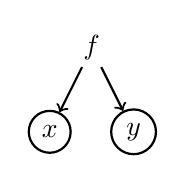
\begin{tikzpicture}[->,thick,scale=.71, every node/.style={scale=1}]
      \tikzstyle{tnode}=[circle, inner sep=.5mm]
      \tikzstyle{var}=[ circle, inner sep=1mm,draw]
      \node[tnode] {$f$}
                child {node[var] {$x$} }
                child {node[var] {$y$} 
                };
  \end{tikzpicture}


  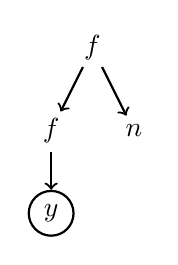
\begin{tikzpicture}[->,thick,scale=.7, every node/.style={scale=1}]
  \tikzstyle{tnode}=[circle, inner sep=.5mm]
  \tikzstyle{var}=[ circle, inner sep=1mm,draw]
  \node[tnode] {$f$}
      child {
        node[tnode] {$f$}
        child {node[var] {$y$} }
      }
      child {node[tnode] {$n$} 
      };
  \end{tikzpicture}
\end{document}

